\def\mybox#1{\hbox{\vrule height 2ex width 0pt depth 0.6ex#1}}
\def\taste[#1]#2{%
  \tikz[x=8mm,y=8mm,baseline=(N.base)] \tasteinnerx[#1]{#2};%
}
\def\tasteinnerx[#1]#2{%
  \node[midway,inner sep=0mm,draw,rounded corners,anchor=base,minimum width=10mm,#1] (N) {\mybox{#2}}%
}
\def\tasteinner[#1]#2{%
  node[midway,inner sep=0mm,draw,rounded corners,minimum width=10mm,#1] (N) {\mybox{#2}}%
}
\def\tasteinnerOK{\tasteinner[fill=green!20]{OK}}
\def\tasteOK{\taste[fill=green!20]{OK}}
\def\tasteC{\taste[fill=red!20]{C}}
\def\tasteinnerC{\tasteinner[fill=red!20]{C}}
\def\tasteRein{\taste[fill=blue!10]{rein}}
\def\tasteinnerRein{\tasteinner[fill=blue!10]{rein}}
\def\tasteZitro{\taste[fill=yellow!10]{zitro}}
\def\tasteinnerZitro{\tasteinner[fill=yellow!10]{zitro}}

\newcommand{\ioeps}[1]{#1|\varepsilon}

\subsection{Mealy-Automat}
\begin{frame}{Der Getränkeautomat}

	\begin{exampleblock}{Beispiel} \small
		Betrachte einen Getränkeautomaten:
		Man kann nur 1-Euro"=Stücke einwerfen und vier Tasten drücken: Es gibt
		zwei Auswahltasten für Mineralwasser \tasteRein{} und Zitronensprudel
		\tasteZitro{}, eine Abbruch"=Taste \tasteC{} und eine \tasteOK-Taste.

	
	\begin{itemize}
	\item Jede Flasche Sprudel kostet 1 Euro.
	\item Es kann ein Guthaben von 1 Euro gespeichert werden. Wirft man
	  weitere Euro"=Stücke ein, werden sie sofort wieder ausgegeben.
	\item Wenn man mehrfach Auswahltasten drückt, wird der letzte Wunsch
	  gespeichert.
	\item Bei Drücken der Abbruch"=Taste wird alles bereits eingeworfenen
	  Geld wieder zurückgegeben und kein Getränkewunsch mehr gespeichert.
	\item Drücken der OK-Taste wird ignoriert, solange noch kein Euro
	  eingeworfen wurde oder keine Getränkesorte ausgewählt wurde.

	  Andernfalls wird das gewünschte Getränk ausgeworfen.
	\end{itemize} 
	\end{exampleblock}
\end{frame}

\begin{frame}{Der Getränkeautomat}

	\begin{exampleblock}{Beispiel}
		\begin{figure}[ht]
  \centering
  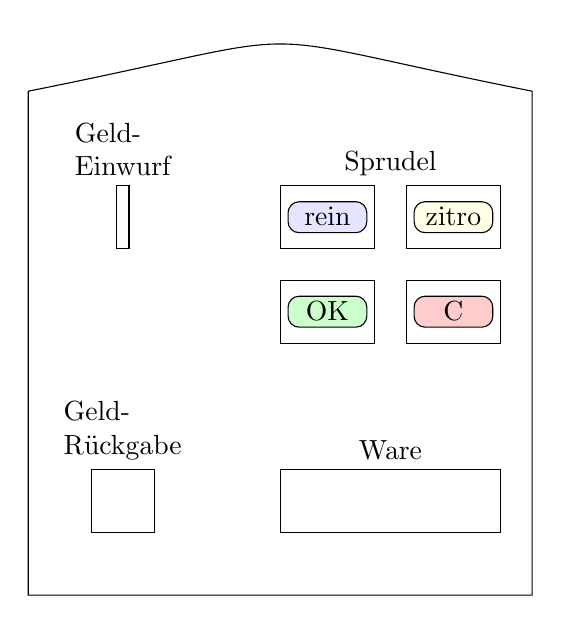
\begin{tikzpicture}[x=8mm,y=8mm]
    % Rahmen
    \draw (0,0) -- (8,0) -- (8,8) .. controls  (3,9) and (5,9) .. (0,8) -- cycle;
    % Geldschlitz 
    \draw (1.4,5.5) rectangle ++(0.2,1) ++(-0.1,0) node[anchor=south] {\vbox{\hbox{Geld-}\hbox{Einwurf}}};
    % Geldrückgabe 
    \draw (1,1) rectangle ++(1,1) ++(-0.5,0) node[anchor=south] {\vbox{\hbox{Geld-}\hbox{Rückgabe}}};
    % Warenauswurf
    \draw (4,1) rectangle ++(3.5,1) ++(-1.75,0) node[anchor=south] {Ware};
    
    % Tasten
    \draw (2.75,3) ++(3,3.5) node[anchor=south] {Sprudel};
    \draw (4,5.5) rectangle ++(1.5,1)\tasteinnerRein;
    \draw (6,5.5) rectangle ++(1.5,1) \tasteinnerZitro;
    \draw (4,4) rectangle ++(1.5,1) \tasteinnerOK;
    \draw (6,4) rectangle ++(1.5,1) \tasteinnerC;
  \end{tikzpicture}
  \caption{Ein primitiver Getr"ankeautomat}
  \label{fig:getraenkeautomat}
\end{figure}
	\end{exampleblock}
\end{frame}

\begin{frame}[fragile]{Der Getränkeautomat}

	\begin{exampleblock}{Beispiel}
		\begin{figure}[ht]
  \centering
  \small
  \begin{tikzpicture}[->,>=stealth]
    \matrix[matrix of math nodes,column sep=25mm,row sep=20mm,nodes={circle,draw,inner sep=1pt}]   {
      |(0-)| (0,-) & |(0R)| (0,R) & |(0Z)| (0,Z) \\
      |(1-)| (1,-) & |(1R)| (1,R) & |(1Z)| (1,Z) \\
    };

    \coordinate[left of=0-] (start);

    \draw (start) -- node[auto] {} (0-);

    % Schleifen
    \draw (0-) edge[loop above]  node[pos=0.5] {$\ioeps{O}$,$\ioeps{C}$} ();
    \draw (0R) edge[loop above] node[pos=0.9,anchor=west] {$\ioeps{R}$,$\ioeps{O}$} ();
    \draw (0Z) edge[loop above] node[pos=0.5] {$\ioeps{Z}$,$\ioeps{O}$} ();
    \draw (1-) edge[loop below]  node[pos=0.5] {$\io{1}{1}$,$\ioeps{O}$} ();
    \draw (1R) edge[loop below] node[pos=0.9,anchor=east] {$\io{1}{1}$,$\ioeps{R}$} ();
    \draw (1Z) edge[loop below] node[pos=0.5] {$\io{1}{1}$,$\ioeps{Z}$} ();

    % andere Kanten
    \draw (0-) -- node[right,pos=0.2] {$\ioeps{1}$} (1-);
    \draw (0R) -- node[right,pos=0.2] {$\ioeps{1}$} (1R);
    \draw (0Z) -- node[right,pos=0.2] {$\ioeps{1}$} (1Z);

    \draw (1-) to[bend left=10] node[left,pos=0.2] {$\io{C}{1}$} (0-);

    \draw (0-) to[bend right=10] node[below] {$\ioeps{R}$} (0R);
    \draw (0R) to[bend right=10] node[above,pos=0.1] {$\ioeps{C}$} (0-);
    \draw (0R) to[bend right=10] node[below] {$\ioeps{Z}$} (0Z);
    \draw (0Z) to[bend right=10] node[above] {$\ioeps{R}$} (0R);
    \draw (0-) to[bend left=32]  node[below,pos=0.2] {$\ioeps{Z}$} (0Z);
    \draw (0Z) to[bend right=40] node[above] {$\ioeps{C}$} (0-);

    \draw (1-) to[bend right=10] node[above] {$\ioeps{R}$} (1R);
    \draw (1R) -- node[below,pos=0.4,anchor=north east] {$\io{O}{R}$,$\io{C}{1}$} (0-); %!!
    \draw (1R) to[bend right=10] node[below] {$\ioeps{Z}$} (1Z);
    \draw (1Z) to[bend right=10] node[above] {$\ioeps{R}$} (1R);
    \draw (1-) to[bend left=-32] node[below,pos=0.2] {$\ioeps{Z}$} (1Z);
    \draw (1Z) -- node[above,pos=0.3,anchor=south west] {$\io{O}{Z}$,$\io{C}{1}$} (0-); %!!
  \end{tikzpicture}
\end{figure}
	\end{exampleblock}
\end{frame}

\begin{frame}{Mealy-Automat}
	\begin{block}{Def.: Mealy-Automat}
		Ein (endlicher) \textbf{Mealy-Automat} $A=(Z, z_0, X, f, Y, g)$ ist bestimmt durch:
		\begin{itemize}
			\item endliche Zustandsmenge $Z$,
			\item Anfangszustand $z_0 \in Z$,
			\item Eingabealphabet $X$,
			\item Zustandsüberführungsfunktion $f: Z \times X \rightarrow Z$,
			\item Ausgabealphabet $Y$,
			\item Ausgabefunktion $g: Z \times X \rightarrow Y^{\ast}$
		\end{itemize}
	\end{block}
\pause
	\begin{alertblock}{Achtung!}
	$f$ ist eine \textbf{Funktion}, also muss man von jedem Zustand mit allen Eingaben ``irgendwohin'' gelangen! Stichwort: Müllzustand.
	\end{alertblock}
\end{frame}



\begin{frame}{Mealy-Automat}
	\begin{block}{Def.: Verallgemeinerte Zustandsübergangsfunktion $f_{\ast}$}
		$f_{\ast} : Z \times X^{\ast} \rightarrow Z$ gibt den Zustand aus, der durch die Eingabe eines Wortes erreicht wird, und ist definiert durch:
		\begin{align*}
			f_{\ast}(z,\varepsilon) &= z \\
			\forall w \in X^{\ast} : \forall x \in X : f_{\ast}(z,wx) &= f(f_{\ast}(z,w),x)\\
		\end{align*}
		Oder als alternative Definition:
		\begin{align*}
			\bar{f}_{\ast}(z,\varepsilon) &= z \\
			\forall w \in X^{\ast} : \forall x \in X : \bar{f}_{\ast}(z,xw) &= \bar{f}_{\ast}(f(z,x),w)
		\end{align*}
	\end{block}
\end{frame}

\begin{frame}{Mealy-Automat}
	\begin{block}{Def.: Verallgemeinerte Zustandsübergangsfunktion $f_{\ast\ast}$}
		$f_{\ast\ast} : Z \times X^{\ast} \rightarrow Z^{\ast}$ gibt \textbf{alle} Zustände aus, die bei der Eingabe eines Wortes durchlaufen werden, und ist definiert durch:
		\begin{align*}
			f_{\ast\ast}(z,\varepsilon) = z\\
			\forall w \in X^{\ast} : \forall x \in X : f_{\ast\ast}(z,wx) &= f_{\ast\ast}(z,w) \cdot f(f_{\ast}(z,w),x)\\
		\end{align*}
	\end{block}
\end{frame}

\begin{frame}[fragile]{Mealy-Automat}

	\begin{exampleblock}{Aufgabe zu $f_{\ast}$ und $f_{\ast\ast}$}
		\begin{columns}
			\begin{column}{0.6\textwidth}
				\begin{figure}[ht]
  \centering
  \tiny
  \begin{tikzpicture}[->,>=stealth]
    \matrix[matrix of math nodes,column sep=20mm,row sep=20mm,nodes={circle,draw,inner sep=1pt}]   {
      |(0-)| (0,-) & |(0R)| (0,R) & |(0Z)| (0,Z) \\
      |(1-)| (1,-) & |(1R)| (1,R) & |(1Z)| (1,Z) \\
    };

    \coordinate[left of=0-] (start);

    \draw (start) -- node[auto] {} (0-);

    % Schleifen
    \draw (0-) edge[loop above]  node[pos=0.5] {$\ioeps{O}$,$\ioeps{C}$} ();
    \draw (0R) edge[loop above] node[pos=0.9,anchor=west] {$\ioeps{R}$,$\ioeps{O}$} ();
    \draw (0Z) edge[loop above] node[pos=0.5] {$\ioeps{Z}$,$\ioeps{O}$} ();
    \draw (1-) edge[loop below]  node[pos=0.5] {$\io{1}{1}$,$\ioeps{O}$} ();
    \draw (1R) edge[loop below] node[pos=0.9,anchor=east] {$\io{1}{1}$,$\ioeps{R}$} ();
    \draw (1Z) edge[loop below] node[pos=0.5] {$\io{1}{1}$,$\ioeps{Z}$} ();

    % andere Kanten
    \draw (0-) -- node[right,pos=0.2] {$\ioeps{1}$} (1-);
    \draw (0R) -- node[right,pos=0.2] {$\ioeps{1}$} (1R);
    \draw (0Z) -- node[right,pos=0.2] {$\ioeps{1}$} (1Z);

    \draw (1-) to[bend left=10] node[left,pos=0.2] {$\io{C}{1}$} (0-);

    \draw (0-) to[bend right=10] node[below] {$\ioeps{R}$} (0R);
    \draw (0R) to[bend right=10] node[above,pos=0.1] {$\ioeps{C}$} (0-);
    \draw (0R) to[bend right=10] node[below] {$\ioeps{Z}$} (0Z);
    \draw (0Z) to[bend right=10] node[above] {$\ioeps{R}$} (0R);
    \draw (0-) to[bend left=32]  node[below,pos=0.2] {$\ioeps{Z}$} (0Z);
    \draw (0Z) to[bend right=40] node[above] {$\ioeps{C}$} (0-);

    \draw (1-) to[bend right=10] node[above] {$\ioeps{R}$} (1R);
    \draw (1R) -- node[below,pos=0.4,anchor=north east] {$\io{O}{R}$,$\io{C}{1}$} (0-); %!!
    \draw (1R) to[bend right=10] node[below] {$\ioeps{Z}$} (1Z);
    \draw (1Z) to[bend right=10] node[above] {$\ioeps{R}$} (1R);
    \draw (1-) to[bend left=-32] node[below,pos=0.2] {$\ioeps{Z}$} (1Z);
    \draw (1Z) -- node[above,pos=0.3,anchor=south west] {$\io{O}{Z}$,$\io{C}{1}$} (0-); %!!
  \end{tikzpicture}
\end{figure}
			\end{column}
			\begin{column}{0.375\textwidth}
			\small
				Gib an:
				\begin{enumerate}
					\item $f_{\ast}((0,-), R1O)$
					\item $f_{\ast\ast}((0,-), R1O)$
					\item $f_{\ast}((0,-), C1Z)$
					\item $f_{\ast\ast}((0,-), RZO)$
					\item $f_{\ast\ast}((1,Z), RZO)$
					\item $f_{\ast}((0,-), RZ1R1C1ZO)$
				\end{enumerate}
			\end{column}
		\end{columns}
	\end{exampleblock}
\end{frame}

\begin{frame}{Mealy-Automat}
	\begin{block}{Lösung zur Aufgabe zu $f_{\ast}$ und $f_{\ast\ast}$}
		\begin{enumerate}
					\item $f_{\ast}((0,-), R1O) = (0,-)$
					\item $f_{\ast\ast}((0,-), R1O) = (0,-)(0,R)(1,R)(0,-)$
					\item $f_{\ast}((0,-), C1Z) = (1,Z)$
					\item $f_{\ast\ast}((0,-), RZO) = (0,-)(0,R)(0,Z)(0,Z)$
					\item $f_{\ast\ast}((1,Z), RZO) = (1,Z)(1,R)(1,Z)(0,-)$
					\item $f_{\ast}((0,-), RZ1R1C1ZO)= (0,-)$
				\end{enumerate}
	\end{block}
\end{frame}

\begin{frame}{Mealy-Automat}
	\begin{block}{Def.: Verallgemeinerte Ausgabefunktion $g_{\ast}$}
		$g_{\ast} : Z \times X^{\ast} \rightarrow Z$ gibt die letzte Ausgabe aus, die durch die Eingabe eines Wortes produziert wird, und ist definiert durch:
		\begin{align*}
			g_{\ast}(z,\varepsilon) &= \varepsilon \\
			\forall w \in X^{\ast} : \forall x \in X : g_{\ast}(z,wx) &= g(f_{\ast}(z,w),x)\\
		\end{align*}
	\end{block}

	\begin{block}{Def.: Verallgemeinerte Ausgabefunktion $g_{\ast\ast}$}
		$g_{\ast\ast} : Z \times X^{\ast} \rightarrow Z^{\ast}$ gibt \textbf{alle} Ausgaben konkateniert aus, die bei der Eingabe eines Wortes erzeugt werden, und ist definiert durch:
		\begin{align*}
			g_{\ast\ast}(z,\varepsilon) = \varepsilon\\
			\forall w \in X^{\ast} : \forall x \in X : g_{\ast\ast}(z,wx) &= g_{\ast\ast}(z,w) \cdot g_{\ast}(z,wx)\\
		\end{align*}
	\end{block}
\end{frame}

\begin{frame}[fragile]{Mealy-Automat}

	\begin{exampleblock}{Aufgabe zu $g_{\ast}$ und $g_{\ast\ast}$}
		\begin{columns}
			\begin{column}{0.6\textwidth}
				\begin{figure}[ht]
  \centering
  \tiny
  \begin{tikzpicture}[->,>=stealth]
    \matrix[matrix of math nodes,column sep=20mm,row sep=20mm,nodes={circle,draw,inner sep=1pt}]   {
      |(0-)| (0,-) & |(0R)| (0,R) & |(0Z)| (0,Z) \\
      |(1-)| (1,-) & |(1R)| (1,R) & |(1Z)| (1,Z) \\
    };

    \coordinate[left of=0-] (start);

    \draw (start) -- node[auto] {} (0-);

    % Schleifen
    \draw (0-) edge[loop above]  node[pos=0.5] {$\ioeps{O}$,$\ioeps{C}$} ();
    \draw (0R) edge[loop above] node[pos=0.9,anchor=west] {$\ioeps{R}$,$\ioeps{O}$} ();
    \draw (0Z) edge[loop above] node[pos=0.5] {$\ioeps{Z}$,$\ioeps{O}$} ();
    \draw (1-) edge[loop below]  node[pos=0.5] {$\io{1}{1}$,$\ioeps{O}$} ();
    \draw (1R) edge[loop below] node[pos=0.9,anchor=east] {$\io{1}{1}$,$\ioeps{R}$} ();
    \draw (1Z) edge[loop below] node[pos=0.5] {$\io{1}{1}$,$\ioeps{Z}$} ();

    % andere Kanten
    \draw (0-) -- node[right,pos=0.2] {$\ioeps{1}$} (1-);
    \draw (0R) -- node[right,pos=0.2] {$\ioeps{1}$} (1R);
    \draw (0Z) -- node[right,pos=0.2] {$\ioeps{1}$} (1Z);

    \draw (1-) to[bend left=10] node[left,pos=0.2] {$\io{C}{1}$} (0-);

    \draw (0-) to[bend right=10] node[below] {$\ioeps{R}$} (0R);
    \draw (0R) to[bend right=10] node[above,pos=0.1] {$\ioeps{C}$} (0-);
    \draw (0R) to[bend right=10] node[below] {$\ioeps{Z}$} (0Z);
    \draw (0Z) to[bend right=10] node[above] {$\ioeps{R}$} (0R);
    \draw (0-) to[bend left=32]  node[below,pos=0.2] {$\ioeps{Z}$} (0Z);
    \draw (0Z) to[bend right=40] node[above] {$\ioeps{C}$} (0-);

    \draw (1-) to[bend right=10] node[above] {$\ioeps{R}$} (1R);
    \draw (1R) -- node[below,pos=0.4,anchor=north east] {$\io{O}{R}$,$\io{C}{1}$} (0-); %!!
    \draw (1R) to[bend right=10] node[below] {$\ioeps{Z}$} (1Z);
    \draw (1Z) to[bend right=10] node[above] {$\ioeps{R}$} (1R);
    \draw (1-) to[bend left=-32] node[below,pos=0.2] {$\ioeps{Z}$} (1Z);
    \draw (1Z) -- node[above,pos=0.3,anchor=south west] {$\io{O}{Z}$,$\io{C}{1}$} (0-); %!!
  \end{tikzpicture}
\end{figure}
			\end{column}
			\begin{column}{0.4\textwidth}
			\small
				Gib an:
				\begin{enumerate}
					\item $g_{\ast}((0,-), R1O)$
					\item $g_{\ast\ast}((0,-), R1O)$
					\item $g_{\ast\ast}((0,-), R11O)$
					\item $g_{\ast}((0,-), C1Z)$
					\item $g_{\ast\ast}((0,-), RZO)$
					\item $g_{\ast\ast}((1,Z), RZO)$
					\item $g_{\ast\ast}((0,-), RZ1R1C1ZO)$
				\end{enumerate}
			\end{column}
		\end{columns}
	\end{exampleblock}
\end{frame}

\begin{frame}{Mealy-Automat}
	\begin{block}{Lösung zur Aufgabe zu $g_{\ast}$ und $g_{\ast\ast}$}
		\begin{enumerate}
					\item $g_{\ast}((0,-), R1O) = R$
					\item $g_{\ast\ast}((0,-), R1O) = R$
					\item $g_{\ast\ast}((0,-), R11O) = 1R$
					\item $g_{\ast}((0,-), C1Z) = \varepsilon$
					\item $g_{\ast\ast}((0,-), RZO) = \varepsilon$
					\item $g_{\ast\ast}((1,Z), RZO) = Z $
					\item $g_{\ast\ast}((0,-), RZ1R1C1ZO)= 11Z$
				\end{enumerate}
	\end{block}
\end{frame}



\subsection{Moore-Automat}
\begin{frame}{Moore-Automat}
	\begin{block}{Def.: Moore-Automat}
		Ein (endlicher) \textbf{Moore-Automat} $A=(Z, z_0, X, f, Y, h)$ ist bestimmt durch:
		\begin{itemize}
			\item endliche Zustandsmenge $Z$,
			\item Anfangszustand $z_0 \in Z$,
			\item Eingabealphabet $X$,
			\item Zustandsüberführungsfunktion $f: Z \times X \rightarrow Z$,
			\item Ausgabealphabet $Y$,
			\item Ausgabefunktion $h: Z \rightarrow Y^{\ast}$
		\end{itemize}

	Der Unterschied zum Mealy Automaten ist also , dass die Ausgabe nur vom Zustand abhängt, nicht von der Eingabe.

	\end{block}
\end{frame}

\begin{frame}[fragile]{Moore-Automat}
	\begin{exampleblock}{Beispiel}
		\begin{figure}[ht]
  \centering
  \begin{tikzpicture}[shorten >=1pt,node distance=2cm,auto,initial text=,->,>=stealth]
   \node[state,initial]  (q_0)                       {$q_{\varepsilon}\!\mid\! 0$};
   \node[state]          (q_1) [above right of= q_0] {$q_{a}\!\mid\! 0$};
    \node[state]          (q_2) [below right of= q_0] {$q_{b}\!\mid\! 0$};
   \node[state](q_3) [below right of=q_1] {$q_f\!\mid\! 1$};
   \node[state](q_4) [right of=q_3] {$q_r\!\mid\! 0$};
    \path[->] (q_0) edge              node        {$a$} (q_1)
                    edge              node [swap] {$b$} (q_2)
              (q_1) edge              node        {$b$} (q_3)
                    edge [loop above] node        {$a$} ()
              (q_2) edge              node [swap] {$a$} (q_3)
                    edge [loop below] node        {$b$} ()
              (q_3) edge              node        {$a,b$} (q_4)
              (q_4) edge [loop above] node        {$a,b$} ();
  \end{tikzpicture}
\end{figure}
	\end{exampleblock}
\end{frame}

\begin{frame}{Moore-Automat}
	\begin{block}{Def.: Verallgemeinerte Zustandsübergangsfunktionen $f_{\ast}$ und $f_{\ast\ast}$}
		Wie bei Mealy-Automaten.
	\end{block}

	\begin{block}{Def.: Verallgemeinerte Ausgabenfunktion $g_{\ast} = h \circ f_{\ast}$}
		$g_{\ast} : Z \times X^{\ast} \rightarrow Y$ gibt die letzte Ausgabe aus und ist definiert durch:
		\[
			\forall(z,w) \in Z \times X^{\ast} : g_{\ast}(z,w) = h(f_{\ast}(z,w))
		\]
	\end{block}

	\begin{block}{Def.: Verallgemeinerte Ausgabenfunktion $g_{\ast\ast} = h^{\ast\ast} \circ f_{\ast\ast}$}
		$g_{\ast\ast} : Z \times X^{\ast} \rightarrow Y$ gibt alle Ausgaben konkateniert aus und ist definiert durch:
		\[
			\forall(z,w) \in Z \times X^{\ast} : g_{\ast\ast}(z,w) = h^{\ast\ast}(f_{\ast\ast}(z,w))
		\]
		mit $h^{\ast\ast} :$\textit{induzierter Homomorphismus von h}.
	\end{block}
\end{frame}

\begin{frame}[fragile]{Moore-Automat}

	\begin{exampleblock}{Aufgabe zu $f_{\ast}$, $f_{\ast\ast}$, $g_{\ast}$ und $g_{\ast\ast}$}
		\begin{columns}
			\begin{column}{0.6\textwidth}
				\begin{figure}[ht]
  \centering
  \small
  \begin{tikzpicture}[shorten >=1pt,node distance=2cm,auto,initial text=,->,>=stealth]
   \node[state,initial]  (q_0)                       {$q_{\varepsilon}\!\mid\! 0$};
   \node[state]          (q_1) [above right of= q_0] {$q_{a}\!\mid\! 0$};
    \node[state]          (q_2) [below right of= q_0] {$q_{b}\!\mid\! 0$};
   \node[state](q_3) [below right of=q_1] {$q_f\!\mid\! 1$};
   \node[state](q_4) [right of=q_3] {$q_r\!\mid\! 0$};
    \path[->] (q_0) edge              node        {$a$} (q_1)
                    edge              node [swap] {$b$} (q_2)
              (q_1) edge              node        {$b$} (q_3)
                    edge [loop above] node        {$a$} ()
              (q_2) edge              node [swap] {$a$} (q_3)
                    edge [loop below] node        {$b$} ()
              (q_3) edge              node        {$a,b$} (q_4)
              (q_4) edge [loop above] node        {$a,b$} ();
  \end{tikzpicture}
\end{figure}
			\end{column}
			\begin{column}{0.4\textwidth}
			\small
				Gib an:
				\begin{enumerate}
					\item $f_{\ast}(q_{\varepsilon}, aab)$
					\item $f_{\ast\ast}(q_{\varepsilon}, aab)$

					\item $g_{\ast}(q_{\varepsilon}, aab)$
					\item $g_{\ast\ast}(q_{\varepsilon}, aab)$
					\item $g_{\ast}(q_{\varepsilon}, abab)$
					\item $g_{\ast\ast}(q_{f}, abab)$
				\end{enumerate}
			\end{column}
		\end{columns}
	\end{exampleblock}
\end{frame}

\begin{frame}{Moore-Automat}
	\begin{block}{Lösung zur Aufgabe zu $f_{\ast}$, $f_{\ast\ast}$, $g_{\ast}$ und $g_{\ast\ast}$}
		\begin{enumerate}
					\item $f_{\ast}(q_{\varepsilon}, aab) = q_{f}$
					\item $f_{\ast\ast}(q_{\varepsilon}, aab) = q_{\varepsilon}q_{a}q_{a}q_{f}$

					\item $g_{\ast}(q_{\varepsilon}, aab) = 1$
					\item $g_{\ast\ast}(q_{\varepsilon}, aab) = 0001$
					\item $g_{\ast}(q_{\varepsilon}, abab) = 0$
					\item $g_{\ast\ast}(q_{f}, abba) = 10000$
			\end{enumerate}
	\end{block}
\end{frame}

\subsection{Akzeptoren}
\begin{frame}{Endlicher Akzeptor}
	\begin{block}{Def.: Endlicher Akzeptor}
		Ein \textbf{endlicher Akzeptor} ist eine Spezialform des Moore-Automaten mit immer genau einem Bit Ausgabe, d.h. $Y = \set{0,1}$ (und $\forall z : h(z) \in Y$).

		Man definiert deshalb eine Menge $F = \setc{z}{h(z)=1}$ der \textbf{akzeptierenden Zustände}.

		Ein endlicher Akzeptor ist also definiert durch:

		\begin{itemize}
			\item endliche Zustandsmenge $Z$,
			\item Anfangszustand $z_0 \in Z$,
			\item Eingabealphabet $X$,
			\item Zustandsüberführungsfunktion $f: Z \times X \rightarrow Z$,
			\item eine Menge akzeptierender Zustände $F \subseteq Z$
		\end{itemize}
		Die von einem endlichen Akzeptor $A$ \textbf{akzeptierte Sprache} ist:
		\[
			L(A) = \setc{w \in X^{\ast}}{f_{\ast}(z_{0},w) \in F}
		\]
	\end{block}
\end{frame}

\begin{frame}[fragile]{Endlicher Akzeptor}
	\begin{exampleblock}{Beispiel}
	\begin{columns}
		\begin{column}{0.6\textwidth}
		\begin{figure}[ht]
  \centering
  \begin{tikzpicture}[shorten >=1pt,node distance=2cm,auto,initial text=,->,>=stealth]
    \node[state,initial]  (q_0)                       {$q_{\varepsilon}$};
    \node[state]          (q_1) [above right of= q_0] {$q_{a}$};
    \node[state]          (q_2) [below right of= q_0] {$q_{b}$};
    \node[state,accepting](q_3) [below right of=q_1] {$q_f$};
    \node[state](q_4) [right of=q_3] {$q_r$};
    \path[->] (q_0) edge              node        {$a$} (q_1)
                    edge              node [swap] {$b$} (q_2)
              (q_1) edge              node        {$b$} (q_3)
                    edge [loop above] node        {$a$} ()
              (q_2) edge              node [swap] {$a$} (q_3)
                    edge [loop below] node        {$b$} ()
              (q_3) edge              node        {$a,b$} (q_4)
              (q_4) edge [loop above] node        {$a,b$} ();
  \end{tikzpicture}
\end{figure}		
		\end{column}
		\begin{column}{0.375\textwidth}
		\centering
		(Akzeptierende Zustände mit Doppelkringel)
		\begin{figure}[ht]
			\begin{tikzpicture}[shorten >=1pt,node distance=2cm,auto,initial text=,->,>=stealth]
				\node[state,accepting] (z) {$z$};
			\end{tikzpicture}
		\end{figure}
		\end{column}
		
	\end{columns}
	\end{exampleblock}
\end{frame}

\begin{frame}{Endlicher Akzeptor}
	\begin{exampleblock}{Aufgabe zu endlichen Akzeptoren}
		\begin{enumerate}
			\small
			\item Zeichne einen Akzeptor mit $X=\set{a,b}$, der alle Wörter akzeptiert, bei denen die Anzahl der \emph{a} durch 5 teilbar ist.
			\item Zeichne einen Akzeptor mit $X=\set{a,b}$, der alle Wörter akzeptiert, in denen nirgends hintereinander zwei \emph{b} vorkommen.
			\item Zeichne einen Akzeptor mit $X=\set{a,b}$, der alle Wörter akzeptiert, in denen irgendwo das Teilwort \emph{abab} vorkommt.
			\item Zeichne einen Akzeptor mit $X=\set{a,b}$, der alle Wörter akzeptiert, in denen nirgends das Teilwort \emph{abab} vorkommt.
			\item Welche Sprache wird vom folgenden Akzeptor $A$ erkannt?
		\end{enumerate}

		\begin{figure}[ht]
  			\centering
  			\begin{tikzpicture}[shorten >=1pt,node distance=2cm,auto,initial text=,->,>=stealth]
   			 	\node[state,initial]  (s_0)                       {$s_{0}$};
  			 	\node[state,accepting](s_1) [right of= s_0] {$s_{1}$};
  			 	\node[state]          (s_2) [right of= s_1] {$s_{2}$};
    			\node[state,accepting](s_3) [right of= s_2] {$s_3$};
    			\draw[->] 	(s_0) 	edge              	node        {$a,b$} (s_1);
              	\draw[->]	(s_1) 	to [bend left=20] 	node        {$a,b$} (s_2);
              	\draw[->]	(s_2) 	to [bend left=20] 	node 		{$b$} 	(s_3);
              	\draw[->]	(s_2)	to [bend left=20] 	node 		{$a$} 	(s_1);
              	\draw[->]	(s_3)	to [bend left=20] 	node 		{$a,b$} (s_2);
  \end{tikzpicture}
\end{figure}	
	\end{exampleblock}
\end{frame}

\begin{frame}{Endlicher Akzeptor}

	\begin{block}{Lösung zur Aufgabe zu endlichen Akzeptoren}
		\begin{enumerate}
			\item siehe Tafel
		\item siehe Tafel
		\item siehe Tafel
		\item siehe Tafel
		\item $L(A)= \setc{w \in \set{a,b}^{\ast}}{\,\setsize{w} mod\, 2 = 1} = \setC{w \in \set{a,b}^{\ast}}{$w$ hat ungerade Länge}$
		\end{enumerate}		
	\end{block}
\end{frame}

\begin{frame}{Endlicher Akzeptor}

	\begin{block}{Lösung}

	1. Zeichne einen Akzeptor mit $X=\set{a,b}$, der alle Wörter akzeptiert, bei denen die Anzahl der \emph{a} durch 5 teilbar ist.\\

	\textbf{Lösung:}\\

	\centering \begin{tikzpicture}[shorten >=1pt,node distance=2cm,auto,initial text=,->,>=stealth]
   		\node[state,initial, accepting] (s_0) {$s_{0}$};
  		\node[state] (s_1) [right of= s_0] {$s_{1}$};
  		\node[state] (s_2) [right of= s_1] {$s_{2}$};
    	\node[state] (s_3) [right of= s_2] {$s_3$};
    	\node[state] (s_4) [right of= s_3] {$s_4$};
    	\draw[->] (s_0) edge node {$a$} (s_1);
    	\draw[->] (s_1) edge node {$a$} (s_2);
    	\draw[->] (s_2) edge node {$a$} (s_3);
    	\draw[->] (s_3) edge node {$a$} (s_4);
    	\draw[->] (s_0) edge node {$a$} (s_1);
    	\draw[->] (s_0) to [loop above] node {$b$} (s_0);
    	\draw[->] (s_1) to [loop above] node {$b$} (s_1);
    	\draw[->] (s_2) to [loop above] node {$b$} (s_2);
    	\draw[->] (s_3) to [loop above] node {$b$} (s_3);
    	\draw[->] (s_4) to [loop above] node {$b$} (s_4);
    	\draw[->] (s_4) to [bend left] node {$b$} (s_0);
 	\end{tikzpicture}
	\end{block}
\end{frame}

\begin{frame}{Endlicher Akzeptor}

	\begin{block}{Lösung}

	2. Zeichne einen Akzeptor mit $X=\set{a,b}$, der alle Wörter akzeptiert, in denen nirgends hintereinander zwei \emph{b} vorkommen.\\

	\textbf{Lösung:}\\

	\centering \begin{tikzpicture}[shorten >=1pt,node distance=2cm,auto,initial text=,->,>=stealth]
   		\node[state,initial,accepting] (s_0) {$s_{0}$};
  		\node[state] (s_1) [right of= s_0] {$s_{1}$};
  		\node[state] (s_2) [right of= s_1] {$s_{2}$};
    	\draw[->] (s_0) to [bend left] node {$b$} (s_1);
    	\draw[->] (s_1) to [bend left] node {$a$} (s_0);
    	\draw[->] (s_1) edge node {$b$} (s_2);
    	\draw[->] (s_0) to [loop above] node {$a$} (s_0);
    	\draw[->] (s_2) to [loop above] node {$a,b$} (s_2);
 	\end{tikzpicture}
	\end{block}
\end{frame}

\begin{frame}{Endlicher Akzeptor}

	\begin{block}{Lösung}

	3. Zeichne einen Akzeptor mit $X=\set{a,b}$, der alle Wörter akzeptiert, in denen irgendwo das Teilwort \emph{abab} vorkommt.\\

	\textbf{Lösung:}\\

	\centering \begin{tikzpicture}[shorten >=1pt,node distance=2cm,auto,initial text=,->,>=stealth]
   		\node[state,initial] (s_0) {$s_{0}$};
  		\node[state] (s_1) [right of= s_0] {$s_{1}$};
  		\node[state] (s_2) [right of= s_1] {$s_{2}$};
    	\node[state] (s_3) [right of= s_2] {$s_3$};
    	\node[state,accepting] (s_4) [right of= s_3] {$s_4$};

    	\draw[->] (s_0) edge node {$a$} (s_1);
    	\draw[->] (s_1) edge node {$b$} (s_2);
    	\draw[->] (s_2) edge node {$a$} (s_3);
    	\draw[->] (s_3) edge node {$b$} (s_4);

    	\draw[->] (s_2) to [bend left] node {$b$} (s_0);
    	\draw[->] (s_3) to [bend right] node[above] {$a$} (s_1);

    	\draw[->] (s_0) to [loop above] node {$b$} (s_0);
    	\draw[->] (s_1) to [loop above] node {$a$} (s_1);
    	\draw[->] (s_4) to [loop above] node {$a,b$} (s_4);
 	\end{tikzpicture}
	\end{block}
\end{frame}

\begin{frame}{Endlicher Akzeptor}

	\begin{block}{Lösung}

	4. Zeichne einen Akzeptor mit $X=\set{a,b}$, der alle Wörter akzeptiert, in denen nirgends das Teilwort \emph{abab} vorkommt.\\

	\textbf{Lösung:}\\

	\centering \begin{tikzpicture}[shorten >=1pt,node distance=2cm,auto,initial text=,->,>=stealth]
   		\node[state,initial,accepting] (s_0) {$s_{0}$};
  		\node[state,accepting] (s_1) [right of= s_0] {$s_{1}$};
  		\node[state,accepting] (s_2) [right of= s_1] {$s_{2}$};
    	\node[state,accepting] (s_3) [right of= s_2] {$s_3$};
    	\node[state] (s_4) [right of= s_3] {$s_4$};

    	\draw[->] (s_0) edge node {$a$} (s_1);
    	\draw[->] (s_1) edge node {$b$} (s_2);
    	\draw[->] (s_2) edge node {$a$} (s_3);
    	\draw[->] (s_3) edge node {$b$} (s_4);

    	\draw[->] (s_2) to [bend left] node {$b$} (s_0);
    	\draw[->] (s_3) to [bend right] node[above] {$a$} (s_1);

    	\draw[->] (s_0) to [loop above] node {$b$} (s_0);
    	\draw[->] (s_1) to [loop above] node {$a$} (s_1);
    	\draw[->] (s_4) to [loop above] node {$a,b$} (s_4);
 	\end{tikzpicture}
	\end{block}
\end{frame}

\begin{frame}{Endlicher Akzeptor}

	\begin{block}{Lösung}
		5. Welche Sprache wird vom folgenden Akzeptor $A$ erkannt?\\

		\begin{figure}[ht]
  			\centering
  			\begin{tikzpicture}[shorten >=1pt,node distance=2cm,auto,initial text=,->,>=stealth]
   			 	\node[state,initial]  (s_0)                       {$s_{0}$};
  			 	\node[state,accepting](s_1) [right of= s_0] {$s_{1}$};
  			 	\node[state]          (s_2) [right of= s_1] {$s_{2}$};
    			\node[state,accepting](s_3) [right of= s_2] {$s_3$};
    			\draw[->] 	(s_0) 	edge              	node        {$a,b$} (s_1);
              	\draw[->]	(s_1) 	to [bend left=20] 	node        {$a,b$} (s_2);
              	\draw[->]	(s_2) 	to [bend left=20] 	node 		{$b$} 	(s_3);
              	\draw[->]	(s_2)	to [bend left=20] 	node 		{$a$} 	(s_1);
              	\draw[->]	(s_3)	to [bend left=20] 	node 		{$a,b$} (s_2);
  			\end{tikzpicture}
			\end{figure}

		\textbf{Lösung:}\\
		\begin{align*}
			L(A) &= \setc{w \in \set{a,b}^{\ast}}{\,|w| mod\, 2 = 1}\\
			&= \setC{w \in \set{a,b}^{\ast}}{$w$ hat ungerade Länge}
		\end{align*}
	\end{block}
\end{frame}